\section{openHAB}
\label{sec:openhab}
    Neben der so eben erläuterten Home Assistant Plattform zählt ebenso die openHAB Plattform als bekannt und 
    in der Anwendung populär. Der \ac{OPENHAB} ist eine Plattform, bei der es sich um eine 
    Softwarelösung handelt, die auf Basis der Programmiersprache Java aufgebaut ist. Die Software steht unter 
    der Eclipse Public License und fällt daher unter die Rubrik der Open-Source Software. Durch die Verwendung 
    von Java ist die Anwendung betriebssystemunabhängig und kann auf beliebigen Betriebssystemen laufen. 
    Ähnlich zu der vorgestellten Home Assistant Software, bietet openHAB ebenso User Interfaces die durch 
    den Webbrowser, Android- und iOS-Geräte unterstützt werden. 
    \\
    \linebreak
    In Kombination mit Java wird bei openHAB das \ac{OSGI}-Framework für die Modularität der Software verwendet. Mit Apache 
    Karaf wird ein Container bereitgestellt, der mit Eclipse Equinox als \acs{OSGI} Laufzeitumgebung agiert. Als 
    \acs{HTTP}-Server ist Jetty in Gebrauch. Die einzelnen Frameworks werden nicht im Detail erläutert, lediglich die für das 
    Verständnis des Konzeptes notwendigen.
    \\
    \linebreak
    Mit openHAB wird eine hochmodulare Software zur Verfügung gestellt, die durch sogenannte \textit{Add-ons} erweitert 
    werden kann. Durch diese wird der Plattform eine breite Palette an Funktionen geboten. Physische Geräte können in 
    großer Anzahl mit der Plattform interagieren und verknüpft werden.\footnote{Einleitung zu openHAB. \url{https://www.openhab.org/docs/} Abgerufen am 25.04.2022}

    \subsection*{Historie}
    \label{sec:historyoHAB}
    Das Smart Home Projekt begann im November 2009 und wurde von Kai Kreuzer entwickelt\footnote{Chronologie und Blogbeiträge von Kai Kreutzer. \url{http://kaikreuzer.blogspot.com} Abgerufen am 28.04.2022.}. 
    Im Februar 2010 wurde das Projekt unter dem Name openHAB bekannt. Nach zweieinhalb jähriger Entwicklung, im Dezember 2012, 
    gab Herrn Kreutzer ein Statement zu der Verwendung von OSGi ab, die seine Überzeugung der Verwendung des Frameworks nach wie 
    vor kundtut.
    \begin{quote}
        „Looking back at this evolution of the project, I am perfectly sure that if I had designed openHAB as a normal Java 
        application instead of an OSGi application, it would not have prospered as it did. It is really the choice of the 
        software architecture that made it happen - and as a nice side effect, the community is not a pure user community 
        as it is the case for many other Open Source projects, but it is full of engaged people who actively contribute to the 
        project.\cite{kaikreutzer2012}“
    \end{quote} 
    Mit der stetig wachsenden Anwendung und deren Community nimmt die Entwicklung des Projekts immer mehr Fahrt auf. 2014 betitelt 
    Kreutzer das Jahr als Jahr des Smart Home, da die Beteiligung, das Interesse und die Entwicklung enorm zunahm und die Community immer 
    großer wurde \cite{kaikreutzer2014}. Seitdem kamen weitere Unterstützungen zu anderen Geräten und 
    Kommunikationsprotokollen dazu. Im Laufe der Entwicklung wurde eine mobile Anwendung entwickelt, mit der die Remotesteuerung 
    implementiert ist. Die Software wird regelmäßig gepatched 

\subsection{Konzept und Architektur}
%\subsection{Architektur}
    Die Steuerungsplattform openHAB bietet vergleichbar zu Home Assistant die Möglichkeit der multifunktionalen Verknüpfung von 
    Geräten und Protokollen. An dieser Stelle werden ebenso mehrere Konzepte verwendet, die die Vereinheitlichung der Plattform 
    verstärkt. Die Konzepte der openHab Software sind in drei größere Rubriken aufgeteilt, die sich wie folgt zusammensetzen:
    \\
    \linebreak
    Die erste Rubrik sind die Dinge (Things), diese sind die Entitäten, die als physische Komponente zu einem System hinzugefügt 
    und viele Funktionalitäten als eines bereitstellen kann. Hierbei ist zu berücksichtigen, dass die sogenannten Dinge nicht 
    immer Geräte sein müssen, diese können auch andere überschaubare Informationsquellen, andere Webdienste und Funktionalitäten 
    darstellen. Aus Sicht des Benutzers sind sie für den Einrichtungs- und Konfigurationsprozess relevant, für den Betrieb 
    jedoch potentiell zu vernachlässigen. Dinge können Konfigurationseigenschaften haben, die optional oder obligatorisch sein 
    können. Solche Eigenschaften können grundlegende Informationen wie eine IP-Adresse, ein Zugriffstoken für einen Webdienst 
    oder eine gerätespezifische Konfiguration sein, die sein Verhalten ändert \cite{openHAB-article}. Mit dem Konzept der Dinge 
    kommen zwei Unterkategorien einher:
    \begin{itemize}
        \item Kanäle (Channels): Jedes Gerät, bzw. Ding stellt Kanäle bereit, mit denen die jeweiligen Funktionen abgebildet werden. 
        An der Stelle an der das physische Gerät angebunden ist, ist der Kanal eine konkrete Funktion dieser Entität. Beispielsweise 
        kann eine Glühbirne einen Kanal für die Farbtemperatur und einen für den Farbwert besitzen. Diese stellen beide die 
        Funktionalität der einen physischen Glühbirne für das System bereit. Grundlegend sind Kanäle mit Elementen verknüpft, mit denen 
        die virtuelle und physische Ebene verbunden wird. Ab dem Zeitpunkt, sobald eine Verbindung hergestellt wird, reagiert ein Ding 
        auf Ereignisse, die für ein Element transferiert werden. Bedingung dafür ist die Verknüpfung zu einem Kanal. Auf der anderen 
        Seite werden aktiv Ereignisse für Objekte gesendet, die mit Kanälen des Dings verknüpft sind \cite{openHAB-article}.
        \item Brücken (Bridges): Die Brücke ist eine besondere Art von Ding. Diese müssen dem System hinzugefügt werden, damit der 
        Zugriff auf andere Dinge ermöglicht wird, bzw. erhalten bleibt. Ein IP-Gateway für Hausautomationssysteme, welches nicht 
        IP-basiert funktioniert, ist eine typisches Beispiel für so eine Brücke.
    \end{itemize}
    An zweiter Stelle stehen die Artikel (Items). Diese Elemente stellen Funktionen dar, die direkt von der Anwendung verwendet 
    werden. Darunter zählen hauptsächlich die Automatisierungslogik oder auch Benutzeroberflächen. Durch Ereignisse werden die 
    Elemente verwendet, da diese einen Zustand besitzen. 
    \\
    Elemente können auch in eine Gruppe zusammengefasst werden. Ein Gruppenelement kann auch Mitglied einer weiteren Gruppe sein. 
    Diese zyklischen Mitgliedschaften sind war nicht verboten, davon wird jedoch abgeraten. Über Benutzeroberflächen können 
    einzelne Gruppenelemente als alleinstehender Eintrag angezeigt werden und eine Navigation zu den jeweiligen Mitgliedern 
    bereitstellen. 
    \\
    \linebreak
    Die dritte große Rubrik sind die Bindungen und Links (Bindings and Links). Diese können als Softwareadapter betrachtet werden, 
    die Dinge für ihr Hausautomationssystem zur Verfügung stellen \cite{openHAB-article}. Aufgabe der Komponente ist die Verknüpfung 
    von Elementen mit physischen Geräten. Um dies zu ermöglichen werden die spezifischen Kommunikationsanforderungen eines Geräts 
    abstrahiert. Dadurch ist eine allgemeinere Behandlung der Komponente durch das Framework möglich. Links stellen das Bindeglied 
    zwischen Dingen und Gegenständen dar. Es ist die Verknüpfung von genau einem Element und einem Kanal. Elemente und 
    Kanäle haben keine eins zu eins Beziehung zueinander. Eine Verknüpfung mit mehreren Komponenten ist auch hier möglich. 
    \\
    \linebreak
    Neben den übergreifenden Konzepten gibt es weitere Konzepte\footnote{Historie und Konzepte von openHAB. \url{https://medium.com/smartsmarthome/openhab-41c30d50fc42} Abgerufen am 28.04.2022}. 
    Diese werden in Folgendem aufgelistet:
    \begin{itemize}
        \item Seitenverzeichnis (Sitemaps): Dies beinhaltet die Konfiguration eines Seitenverzeichnisses, mit dem Schalter, 
        Regler, Texte und vieles mehr hinzugefügt werden kann. Diese Ansichten repräsentieren den Status eines Elements und 
        können darüber gesteuert und überprüft werden.
        \item Regeln (Rules): Eine Regel ist die Verknüpfung eines Ereignisses und einer Aktion. Somit wird nach einem bestimmten 
        Ereignis eine Aktion ausgeführt. Ein Beispiel: Wenn ein Fenster geöffnet wird, soll die Heizung abgeschaltet werden. 
        So lange, bis das Fenster wieder geschlossen wird. 
        \item Persistenz (Persistence): Mit der Persistenzschicht kann festgelegt werden, welche historischen Zustandsereignisse 
        und Informationen gespeichert werden sollen. Dadurch kann nach Systemausfall der Status des Elementes wiederhergestellt werden. 
        \item Modelle (Models): Modelle stellen baumbasierte Gruppierungen von Elementen dar. In der Baumstruktur können Elemente 
        Orte, Punkte und Ausrüstungen sein. Ein Beispiel: Das Wohnzimmer als Standort besteht aus zwei Geräten Heizung und Licht. 
        Die Heizung als Ausstattung hat zwei Punkte: \textit{Ist-Temperatur} und \textit{Soll-Temperatur}.
        \item Seiten (Pages):Alle Seiten und Seitenverzeichnisse kontrollieren die Zustände von Elementen und greifen auf diese zu. 
        Mit openHAB 3 würden weitere Möglichkeiten hinzugefügt, um benutzerdefinierte \acs{UI}, Diagramme, Grundrisse und oder 
        Layouts zu definieren. 
        \item Skripte (Scripts): Skripte sind ähnlich zu den Regeln. Diese spezifizieren eine Aktion und kein Ereignis. Die Skripte 
        können manuell, aber auch über andere Skripte und Regeln ausgeführt werden. 
    \end{itemize}
    Die anfängliche Architektur der openHAB Anwendung teilt sich in drei Sektionen auf: Die Kernkomponenten (blau), das drunter 
    liegende OSGi-Framework (grün) und die Erweiterungen (Add-Ons) (gelb). 
    \begin{figure}[hbt!]
        \centering
        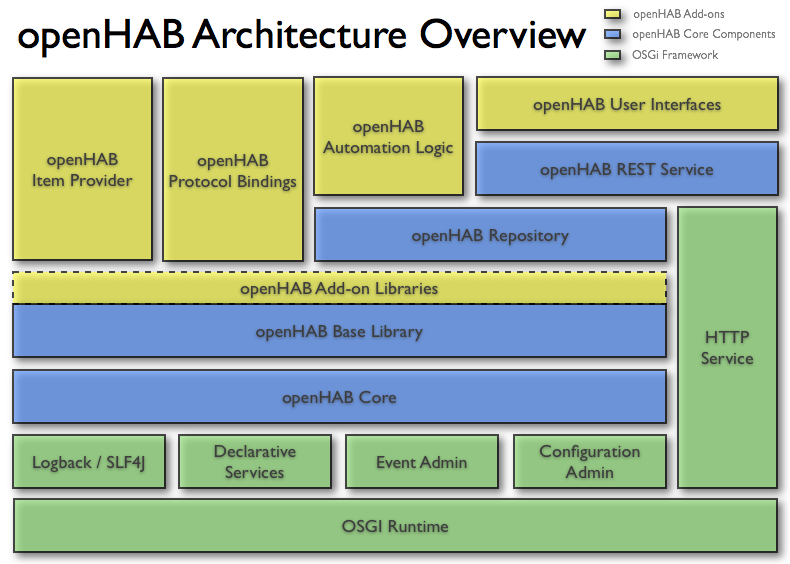
\includegraphics[width=15cm,height=15cm,keepaspectratio]{images/openhab-architecture.png}
        \caption{Architektur der openHAB Plattform \cite{openHAB-architecture2018}}
        \label{fig:architectureopenHAB}
    \end{figure}




\subsection{Ziele und Schwerpunkte}
\subsection{Stärken und Schwächen}

\section{Vergleich von Home Assistant und openHAB}
\label{sec:comparison-HAOS-openHAB}
    %Allgemein gültiger Vergleich (Aufbau, Architektur, Schwerpunkte (Fokus), Umsetzungen, Konnektivität, etc.)
    % https://everythingsmarthome.co.uk/home-assistant-vs-openhab-which-one-is-better/
    % https://smarthome.msuttner.de/openhab-2/vergleich-openhab-vs-home-assistant/ 
    % https://www.electronicshub.org/openhab-vs-home-assistant/ 
    % https://smarthome.university/your-smart-home-platform-home-assistant-vs-openhab/ 

